% !TeX root=../main.tex
\chapter{مفاهیم اولیه و پیش‌زمینه}
% ------------ Section 2.1
\section{دلایل و برتری‌های متن‌باز بودن قرارداد‌های هوشمند}
دلایل زیادی برای متن‌باز نوشتن قراردادهای هوشمند وجود دارد، در ادامه تعدادی از این دلایل توضیح داده می‌شود.

دلیل اول، بلاک‌چین‌ها
\gls{Confidentiality}
ندارند، همه‌ی نود‌های شبکه برای اجرای کد قرارداد هوشمند باید حداقل به
\glspl{bytecode}
قرارداد هوشمند دسترسی داشته باشند و این بایت‌کد‌ها در کاوشگرهای بلاکچین نیز وجود دارند، همچنین
\gls{Decompiler}هایی
وجود دارند که از بایت‌کد‌های قرارداد هوشمند کد سالیدیتی آن را به دست می‌آورند. پس در نتیجه تلاش برای مخفی کردن کدهای قرارداد هوشمند بیهوده خواهد بود.

دلیل دوم، اصلی‌ترین مذیت اپلیکیشن‌های غیرمتمرکز نسبت به اپلیکیشن‌های متمرکز عدم نیاز به اعتماد است، کاربرها می‌توانند کد‌های قرارداد هوشمند را بخوانند و به کد نوشته شده اعتماد کنند،‌در حالی که اگر کد برنامه برای همه کاربران قابل مشاهده نباشد کاربرها باید به سازندگان آن برنامه اعتماد کنند.

دلیل سوم، دیپلوی کردن قرارداد‌های هوشمند معمولاآسان نیست وسرعت تغییرات پایین‌تر از اپلیکیشن‌های متمرکز هست،‌ پس امکان این که با پیدا شدن هر مشکل بتوان به سرعت آن را درست کرد کمتر وجود دارد و مسئله امنیت بسیار اهمیت دارد. متن‌باز نوشتن قرارداد هوشمند باعث می‌شود چشم‌های بیشتری کدهای قرارداد را بخوانند و مشکلات احتمالی سریعتر مشخص و رفع شوند. تعداد زیادی از این پروژه‌ها از همان روز اول قرارداد هوشمند را به صورت متن‌باز توسعه می‌دهند، بعضی نیز ترجیح میدهند که پروژه به مرحله‌ای از توسعه برسد و سپس آن را متن‌باز میکنند.

ر این حوضه سرعت پیشرفت و توسعه به دلیل متن باز بودن به شدت بالاست به نحوی که در طی اجرای این پروژه مرج ریکوئستی روی کتابخانه OpenZeppelin زده شد که در همان روز مرج شد. این موضوع علاوه بر این که نشان‌دهنده سرعت پیشرفت بسیار بالاست، این موضوع را نیز نشان میدهد که در یک جامعه متن‌باز هر توسعه دهنده می‌تواند به پیشرفت جامعه به هر شکلی که می‌تواند کمک کند، اشکالاتی که مشاهده میکند را گزارش دهد یا تصحیح کند.

\begin{figure}[ht]
\centerline{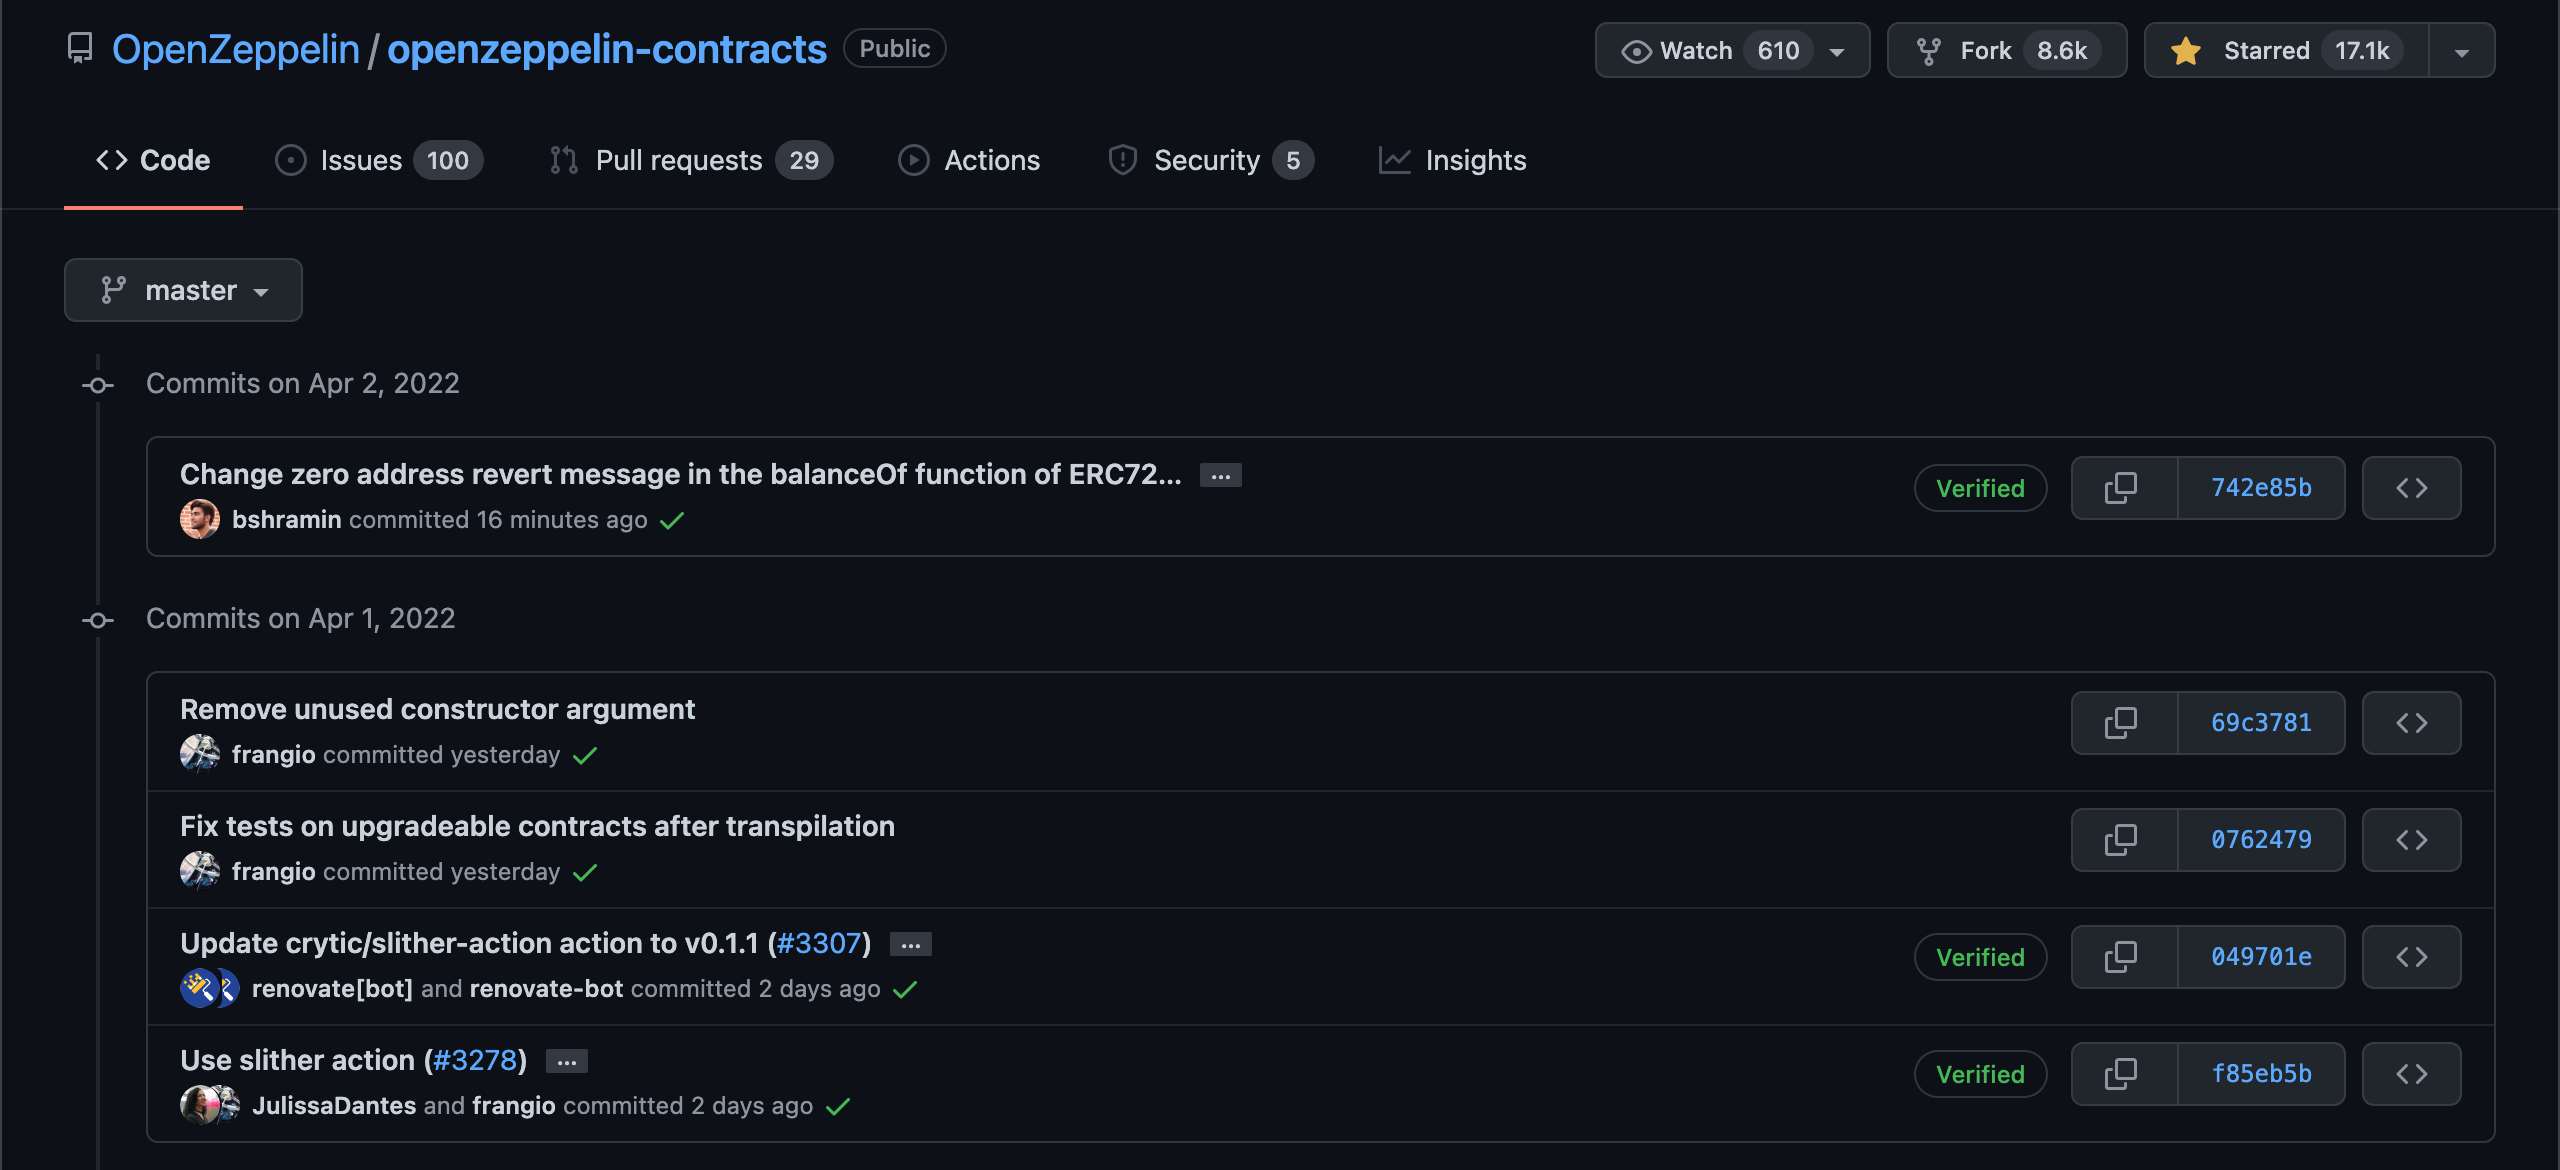
\includegraphics[width=15cm]{OpenZepplinContribution.png}}
\caption{در طی انجام پروژه مرج ریکوئستی روی OpenZeppelin باز شد که در همان روز مرج شد.}
\label{fig:zeppelin-merge-req}
\end{figure}


% ------------ Section 2.2
\section{آشنایی با مفهوم توکن تعویض ناپذیر}
شروع رمزارزها با توکن‌های تعویض پذیر بود، مفهوم تعویض پذیری به این معنی است که یک توکن با توکن دیگر تفاوتی ندارد و با جابه‌جا شدن آن‌ها تغییری ایجاد نمی‌شود. برای مثال یک بیت‌کوین با یک بیت‌کوین دیگر هیچ تفاوتی ندارد.

اما توکن‌های تعویض ناپذیر اینگونه نیستند، هر یک منحصر به فرد است و جابه‌جا کردن آن‌ها با یکدیگر تغییر ایجاد میکند،‌ در دنیای واقعی خانه می‌تواند مثال خوبی از یک دارایی تعویض ناپذیر باشد، هیچ دو خانه‌ای دقیقا شبیه به هم، در یک مکان، در طبقه یکسان و دارای پلاک مشترک نیستند.

پس مثلا به عنوان یک کاربرد، شهرداری می‌تواند یک قرارداد هوشمند ایجاد کند و به هر خانه یک توکن NFT اختصاص دهد. به این صورت صاحب خانه به جای سند یک توکن NFT دارد که مشخص می‌کند که دارایی مطعلق به اوست، و فروش خانه به راحتی انتقال آن NFT به شخص دیگری است.

از نظر فنی هر توکن به این صورت یکتاست که یک TokenId یکتا در قراردادش دارد و هر قرارداد هم دارای یک آدرس یکتا در شبکه بلاکچین است. پس ترکیب Contract Address و TokenId باعث می‌شود که هر توکن یکتا باشد.


% ------------ Section 2.3
\section{کاربردها، حال و آینده}
کاربرد NFTها تا به حال در دو دسته خلاصه می‌شود. دسته اول به عنوان صاحب یک اثر دیجیتال، مانند یک تصویر یا یک موسیقی. دسته دوم به عنوان یک جواز یا بلیت برای ورود به جایی یا دریافت چیزی، برای مثال همایشی برگذار می‌شود که فقط دارندگان NFTهای یک قرارداد هوشمند می‌توانند به آن وارد شوند.

معروف‌ترین پلتفرم معاملاتی این توکن‌ها OpenSea است که می‌توان در آن توکن‌های موجود را مشاهده کرد و یک توکن را توسط مزایده خرید یا به فروش گذاشت. OpenSea در حال حاضر از قراردادهای شبکه‌های اتریوم و سولانا پشتیبانی میکند. دیگر شبکه‌ها نیز معمولا پلتفرم‌های خود را دارند، مانند شبکه Atom که در آن از پلتفرم Stargaze برای معامله NFTها استفاده می‌شود.

کاربردهای NFT ها در آینده می‌تواند بسیار وسیع باشد. دارایی‌های فیزیکی دنیای واقعی، بلیت‌های ورود به یک مکان یا یک همایش، دارایی‌های دنیای مجازی مانند یک موسیقی یا آیتمی در یک بازی و حتی دامنه‌های اینترنتی همه می‌توانند به NFT تبدیل شوند. مزایای تبدیل این موارد به NFT قابلیت نگهداری آسان‌تر، قابلیت فروش و انتقال راحت‌تر، امنیت بیشتر، آزادی در تراکنش‌ها و آشکار بودن مالکیت دارایی بر همگان است.


% ------------ Section 2.4
\section{قرارداد‌های هوشمند و استانداردسازی}
اکثر قرارداد‌های هوشمند قابلیت‌هایی مشابه با یکدیگر دارند، برای مثال گروهی از قرارداد‌های هوشمند توکن‌های تعویض پذیر دارند و گروه توکن‌های تعویض ناپذیر. از طرفی اپلیکیشن‌هایی مانند کیف‌پول‌های دیجیتال، پلتفرم‌های معاملاتی و صرافی‌های نیاز دارند که بتوانند دارایی‌های کاربر اعم از توکن‌های تعویض پذیر و تعویض ناپذیر را ببینند، به همین دلیل باید نحوه صحبت کردن با قراردادهای هوشمند را بدانند.

برای ساده‌تر کردن این فرایند و همسان‌سازی اینترفیس  این قراردادهای هوشمند استانداردهایی تعریف شده است که با استفاده از این استانداردها هم فرایند توسعه اسمارت کانترکت آسان‌تر خواهد شد و هم ارتباط میان قراردادهوشمند و اپلیکیشن‌های دیگر مانند کیف‌پول‌ها، پلتفرم‌های معاملاتی و ... آسان‌تر خواهد شد.

از نمونه‌های معروف این استانداردها
\lr{ERC20}
برای قرارداد‌هایی با توکن‌های تعویض پذیر و
\lr{ERC721}
برای قراردادهایی با توکن‌های تعویض ناپذیر است. در این پروژه از استاندارد
\lr{ERC721}
استفاده می‌شود اما در مورد
\lr{ERC1155}
هم مطالعه شده و توضیح داده می‌شود، به طور خلاصه
\lr{ERC1155}
قابلیت‌های بیشتری از
\lr{ERC721}
دارد و یک قرارداد با این استاندارد می‌تواند هم توکن‌های تعویض پذیر و هم تعویض ناپذیر داشته باشد.

برای استفاده از این استاندارد‌ها از پکیج‌های متن بازی استفاده می‌شود که این استاندارد‌ها را پیاده‌سازی کرده‌اند و از آن‌ها در قراردادی که نوشته می‌شود ارث‌بری می‌شود، یکی از بهترین پیاده‌سازی‌های این استاندارد‌های توسط
\gls{OpenZeppelin}
انجام شده است که در این پروژه نیز از همین پیاده‌سازی استفاده می‌شود.

\subsection{استاندارد \lr{ERC20}}
این استاندارد مناسب توکن‌های تعویض پذیر است. اینترفیسی تعریف می‌کند که نیازهای قراردادهایی با توکن‌های تعویض پذیر را برطرف کند و نحوه تعامل برقرار کردن با آن‌ها را یکسان گرداند. در این استاندارد فقط می‌توان یک نوع توکن تعویض پذیر به تعداد دلخواه داشت. این استاندارد متدهایی برای تعریف حداکثر تعداد توکن‌های موجود، گرفتن موجودی یک آدرس، و انتقال توکن‌ها دارد. توضیحات دقیق‌تر در مورد این استاندارد را می‌توان در وبسایت
اتریوم
\LTRfootnote{\url{https://ethereum.org/en/developers/docs/standards/tokens/erc-20}}
یا اپن‌زپلین
\LTRfootnote{\url{https://docs.openzeppelin.com/contracts/4.x/api/token/erc20}}
مشاهده کرد.

\subsection{استاندارد \lr{ERC721}}
استفاده از استاندارد
\lr{ERC721}
برای توکن‌های تعویض ناپذیر بسیار مرسوم است. در این استاندارد متدها و ایونت‌هایی برای یکسان سازی اینترفیس قراردادهای دارای توکن‌های تعویض ناپذیر تعریف شده است. در این نوع قرارداد‌ها میتوان به تعداد دلخواه توکن‌های متفاوت با یکدیگر داشت، هر توکن یک آیدی یکتا دارد که می‌تواند به صورت ترتیبی یا غیر ترتیبی ایجاد شود.

همچنین متدی وجود دارد که میتواند آیدی یک توکن را به آدرسی تبدیل کند که اطلاعات آن توکن در آنجا موجود است. کاربرها می‌توانند توکن‌هایی که دارند را مشاهده کنند، به یکدیگر ارسال کنند یا به آدرس دیگری وکالت بدهند که توکن‌ها را به شخص دیگری ارسال کند.

تنها قابلیتی که به طور مشخص در این قرارداد معین نشده است که چگونه باید انجام شود قابلیت
\gls{Mint}
توکن‌ها است. اکثر قراردادهای هوشمندی که توکن‌های تعویض ناپذیر دارند به کاربران اجازه ساخت توکن‌ها را نمی‌دهند و ساخت توکن‌ها فقط به آدرس صاحب قرارداد محدود می‌شود. اما در کاپو اینگونه نیست و هرکسی می‌تواند برای خودش توکن بسازد.

اطلاعات دقیق‌تر در مورد این استاندارد را نیز می‌توان در وبسایت
اتریوم
\LTRfootnote{\url{https://ethereum.org/en/developers/docs/standards/tokens/erc-721}}
یا
اپن‌زپلین
\LTRfootnote{\url{https://docs.openzeppelin.com/contracts/4.x/api/token/erc721}}
مشاهده کرد.


\subsection{استاندارد \lr{ERC1155}}
تا اینجا با معروف‌ترین استاندارد‌های موجود برای قراردادهایی که توکن‌های تعویض پذیر یا تعویض ناپذیر دارند آشنا شدیم. اما همچنان نیازمندی‌هایی وجود دارند که توسط هیچ‌یک از این استانداردها برطرف نمی‌شوند. نیازمندی‌هایی مانند:
\begin{itemize}
	\item
داشتن توکن‌های NFT با تعداد محدود به جای فقط یکی.
	\item
داشتن همزمان چندین نوع توکن مختلف در یک قرارداد.
	\item
انتقال همزمان چند توکن از انواع مختلف از کاربری به کاربر دیگر.
\end{itemize}

یک مثال از کاربردی که به این قابلیت‌ها نیاز دارد می‌تواند یک بازی مثل مونوپولی باشد که در آن هر کاربر مقداری پول دارد که در واقع یک توکن تعویض پذیر هست، به عنوان دارایی چند خانه دارد که به عنوان توکن‌های تعویض ناپذیری هستند که از هرکدام فقط یکی وجود دارد و ممکن است چند کارت خروج از زندان داشته باشد که یکتا نیستند اما تعداد محدودی در بازی وجود دارد. استاندارد
\lr{ERC1155}
همه‌ی این نیازها را برطرف می‌کند. همه‌ی این چند نوع توکن می‌توانند همزمان در یک قرارداد هوشمند وجود داشته باشند.

در این استاندارد متدهایی برای تعریف نوعی توکن با تعداد مشخص وجود دارد. اگر نیاز به توکنی تعویض ناپذیر باشد تعداد آن یک قرارداده می‌شود. همچنین متدهایی برای ارسال تعداد مشخص از چند نوع توکن مختلف در یک تراکنش، دادن وکالت توکن‌ها به آدرس دیگر و گرفتن موجودی یک آدرس در این استاندارد وجود دارد.

اطلاعات دقیق‌تر در مورد این استاندارد را نیز می‌توان در وبسایت
اتریوم
\LTRfootnote{\url{https://ethereum.org/en/developers/docs/standards/tokens/erc-1155}}
یا
اپن‌زپلین
\LTRfootnote{\url{https://docs.openzeppelin.com/contracts/4.x/api/token/erc1155}}
مشاهده کرد.
